\documentclass{article}
\usepackage[main=spanish, provide=*]{babel}
\usepackage{xcolor}
\usepackage{array}
\usepackage{graphicx}
\usepackage{tikz}
\usepackage{circuitikz}
\usepackage{pgfplots}
\usepackage{darkmode}
\usepackage{amsmath}
\usepackage[a4paper, top=2cm, bottom=2cm]{geometry}

\enabledarkmode

\definecolor{c1}{HTML}{8bb6e7}
\definecolor{c2}{HTML}{87f3dd}
\definecolor{c3}{HTML}{fdef83}
\definecolor{c4}{HTML}{fdc373}
\definecolor{c5}{HTML}{fd8581}
\definecolor{c6}{HTML}{c573e7}
\definecolor{c7}{HTML}{afdb68}
\definecolor{c8}{HTML}{e59f8b}

\definecolor{page}{HTML}{262626}
\pagecolor{page}

\begin{document}
\title{Respuesta en frecuencia de un amplificador}
\author{Mario López Sáez}
\date{\today}
\maketitle

\begin{center}

\begin{tikzpicture}
    \fill[c1] (0, 0) rectangle ++(1, 0.05);
    \fill[c2] (1, 0) rectangle ++(1, 0.05);
    \fill[c3] (2, 0) rectangle ++(1, 0.05);
    \fill[c4] (3, 0) rectangle ++(1, 0.05);
    \fill[c5] (4, 0) rectangle ++(1, 0.05);
    \fill[c6] (5, 0) rectangle ++(1, 0.05);
    \fill[c7] (6, 0) rectangle ++(1, 0.05);
    \fill[c8] (7, 0) rectangle ++(1, 0.05);
\end{tikzpicture}

\end{center}

\section{Función de transferencia}
La función de transferencia de un circuito \( A(j\omega) \) es una función compleja que representa la respuesta en frecuencia del mismo. A cada pulsación o frecuencia (\(\omega = 2\pi f\)) le corresponde un número complejo cuyo módulo nos indica la respuesta en amplitud (factor ganancia) y su argumento la respuesta de fase (desplazamiento temporal).

\begin{figure}[h!]
    \centering
    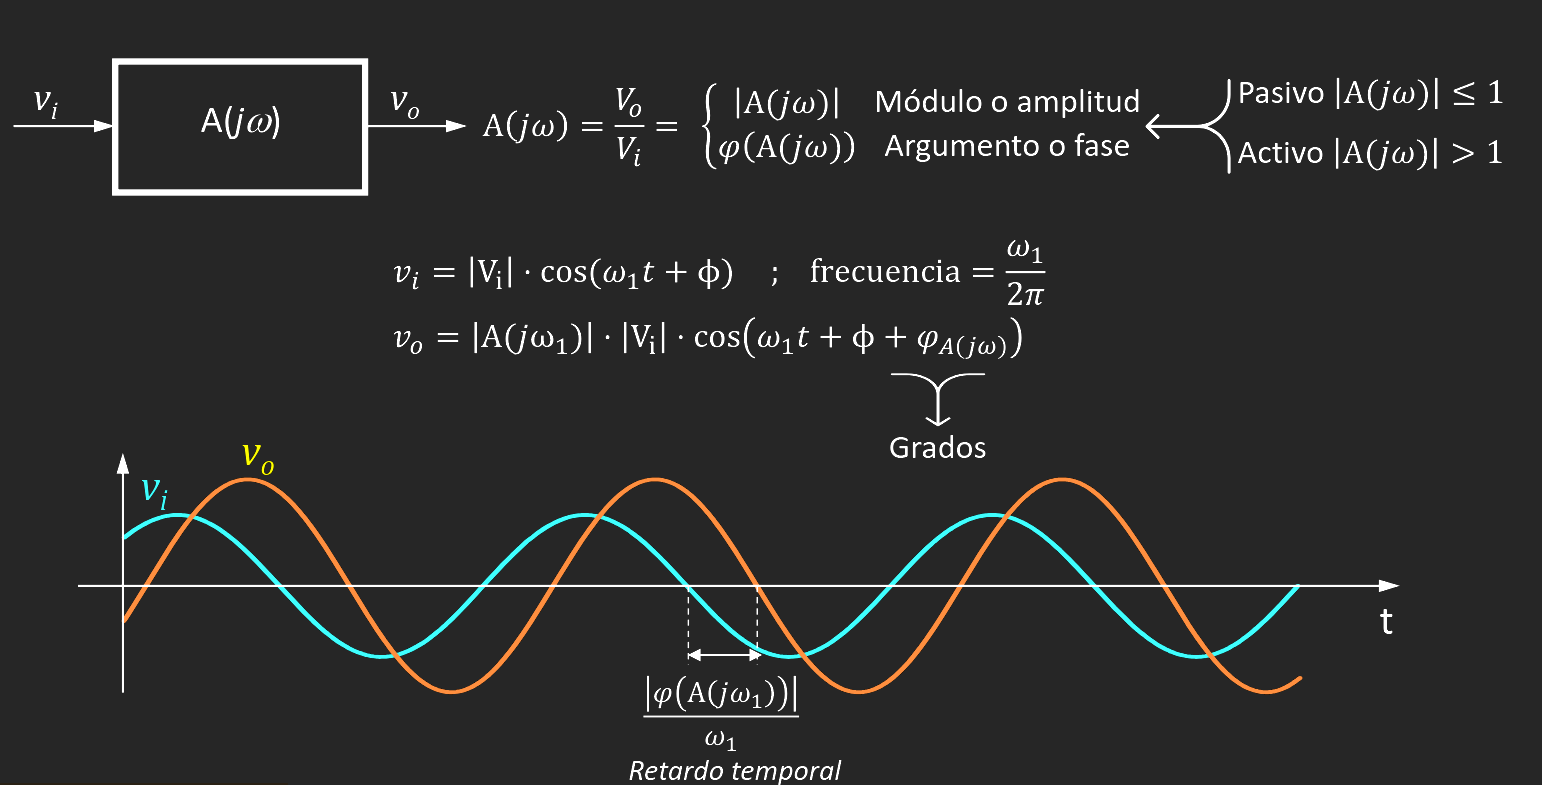
\includegraphics[width=0.9\textwidth]{fig1.jpg} 
\end{figure}
\begin{center}
\textbf{Expresión general de una FDT.} Es un cociente de polinomios con variable $j \omega$
\end{center}
\[ A(j\omega) = \frac{N(j\omega)}{D(j\omega)} = \frac{A_1 + A_2 j\omega + A_3 (j\omega)^2 + A_4 (j\omega)^3 + \ldots + A_{n+1} (j\omega)^n}{B_1 + B_2 j\omega + B_3 (j\omega)^2 + B_4 (j\omega)^3 + \ldots + B_{m+1} (j\omega)^m} \]

\subsection{Ejemplo 1. Filtro paso bajo}

\begin{figure}[h!]
    \centering
    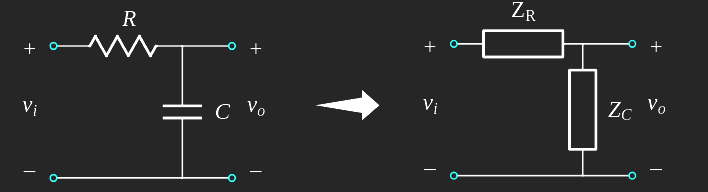
\includegraphics[width=0.9\textwidth]{fig2.jpg} 
\end{figure}
\begin{minipage}{0.5\textwidth}
$$
Z_{R} = R ; \ Z_{C} = \frac{1}{j \omega C}
$$
\[ A(j\omega) = \frac{v_o}{v_i} = \frac{Z_C}{Z_R + Z_C} = \frac{1}{1 + j \omega RC} = \frac{1}{1 + j \frac{\omega}{\omega_0}} \]
\end{minipage}%
\begin{minipage}{0.4\textwidth}
$$
\omega_0 = \frac{1}{R_{1}C_{1}} = \frac{1}{\tau} 
$$
$$
\text{Constante de tiempo } \tau
$$
\end{minipage}


\newpage
\begin{minipage}{0.5\textwidth}
$$
A (j \omega) = \frac{1}{1 + j \omega RC}
$$
\end{minipage}
\begin{minipage}{0.5\textwidth}
    $$
A_{1} = 1, A_{2} = 0, A_{3} = 0 ...
    $$
    $$
B_{1} = 1, B_{2} = RC, B_{3} = 0 ...
    $$
\end{minipage}
\smallskip
\hrule
\smallskip
$$
\text{Amplitud: } |A (j \omega)| = \frac{1}{\sqrt{1 + (\omega RC)^2}}
$$
$$
\text{Fase: } \varphi_A (j \omega) = - \text{arctg}(\omega RC) 
$$

\section{Representación de la FDT. Diagramas de Bode}
\textbf{Diagrama de Bode: }representación de la amplitud y fase de una FDT
\bigskip

\begin{minipage}{0.49\textwidth}
    \centering
    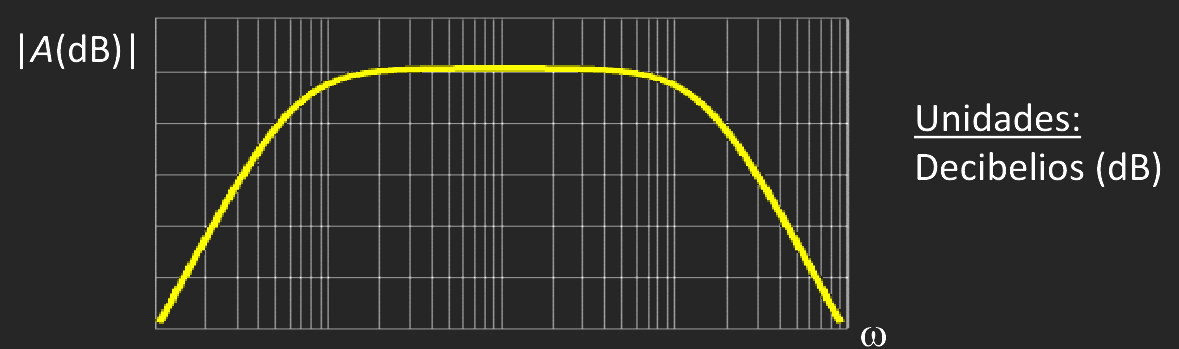
\includegraphics[width=\textwidth]{figbode1.jpg} 
\end{minipage}
\begin{minipage}{0.49\textwidth}
    \centering
    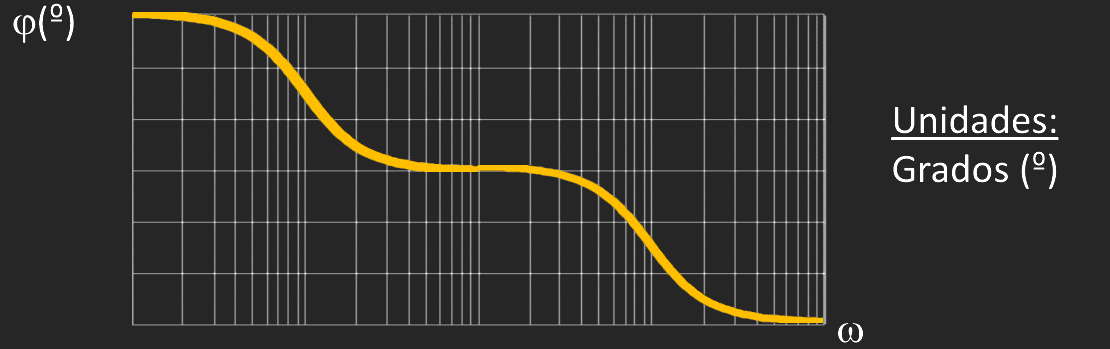
\includegraphics[width=\textwidth]{figbode2.jpg} 
\end{minipage}
\subsection{Factor constante}
$$
A (j \omega) = K_{1}
$$
\begin{minipage}{0.49\textwidth}
$$
|A (j \omega)| = |K_{1}| \to |A (j \omega)|_{dB} = 20 \log |K_{1}|
$$
    \centering
    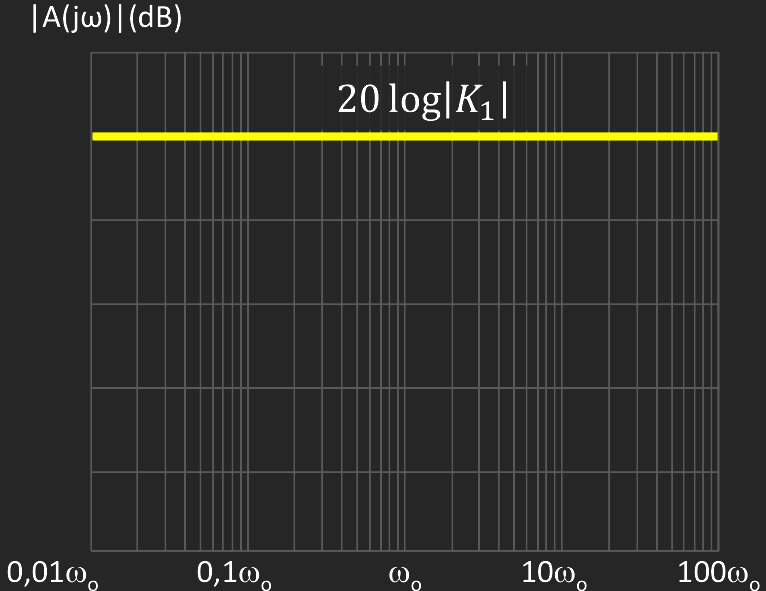
\includegraphics[width=\textwidth]{figbode21.jpg} 
\end{minipage}
\begin{minipage}{0.49\textwidth}
	$$
\varphi [A (j \omega)] = 
\begin{cases}
0^\circ & \text{si } K_{1} > 0 \\
180^\circ & \text{si } K_{1} < 0 
\end{cases}
	$$
    \centering
    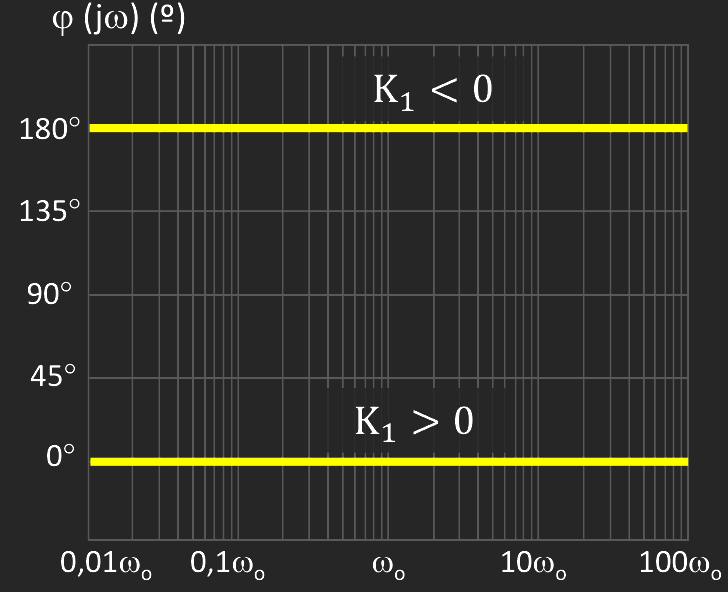
\includegraphics[width=\textwidth]{figbode211.jpg} 
\end{minipage}
\hrule
\subsection{Derivador puro}
$$
A (j \omega) = j \frac{\omega}{\omega_0}
$$
\begin{minipage}{0.45\textwidth}
$$
|A (j \omega)| = \frac{\omega}{\omega_0} \to |A (j \omega)|_{dB} = 20 \log \left(\frac{\omega}{\omega_0}\right)
$$
    \centering
    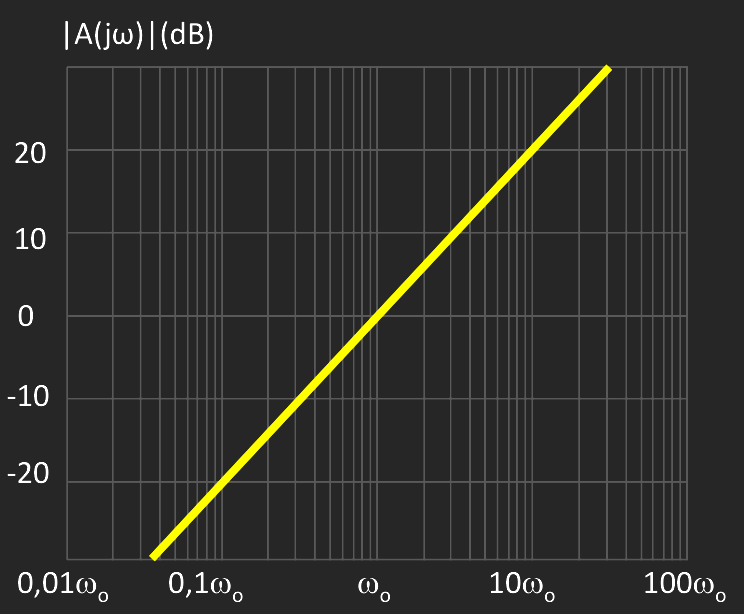
\includegraphics[width=\textwidth]{figbode221.jpg} 
\end{minipage}
\begin{minipage}{0.45\textwidth}
\vspace{-2cm}
$$
\varphi [A (j \omega)] = 90^\circ
$$

\vspace{1cm}

$$
|A (j \omega_0)| = 0 dB \ \ \ |A (j 10 \omega_0)| = 20 dB
$$
$$
\text{Recta de pendiente } +20 \frac{dB}{dec}
$$
\end{minipage}
\newpage
\begin{minipage}{0.49\textwidth}
\textbf{La salida es proporcional a la derivada de la entrada}
$$
v_{i} = A \sin (\omega t)
$$
    \centering
    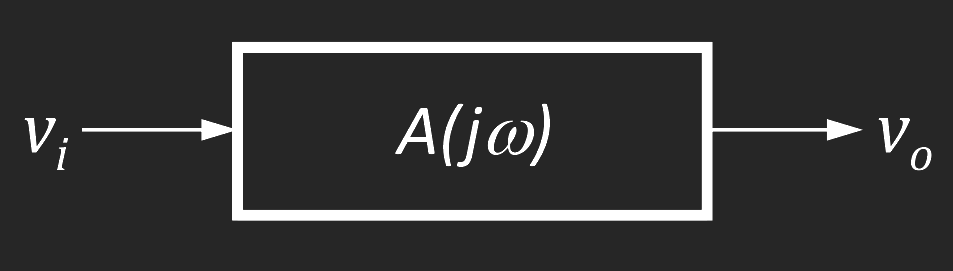
\includegraphics[width=0.5\textwidth]{bloquefdt.jpg} 
$$
v_{o} = \frac{\omega}{\omega_0} A \sin (\omega t + 90^\circ) = A \frac{\omega}{\omega_0} \cos (\omega t)
$$
$$
v_{0} (t) = \frac{dv_i (t)}{dt}
$$
\end{minipage}
\begin{minipage}{0.49\textwidth}
    \centering
    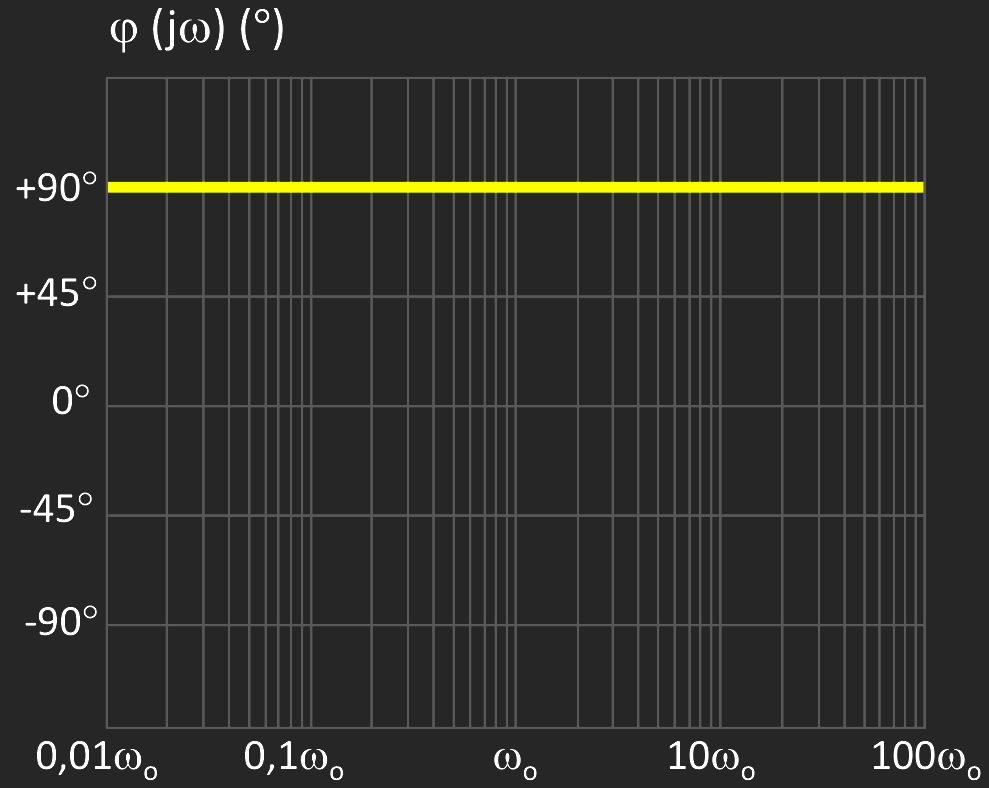
\includegraphics[width=\textwidth]{figbode222.jpg} 
\end{minipage}
\hrule
\subsection{Integrador puro}
$$
A (j \omega) = \frac{1}{j \frac{\omega}{\omega_0}}
$$
\begin{minipage}{0.49\textwidth}
$$
|A (j \omega)| = \frac{1}{\frac{\omega}{\omega_0}} \to |A (j \omega)|_{dB} = 0 - 20 \log \frac{\omega}{\omega_0}
$$
    \centering
    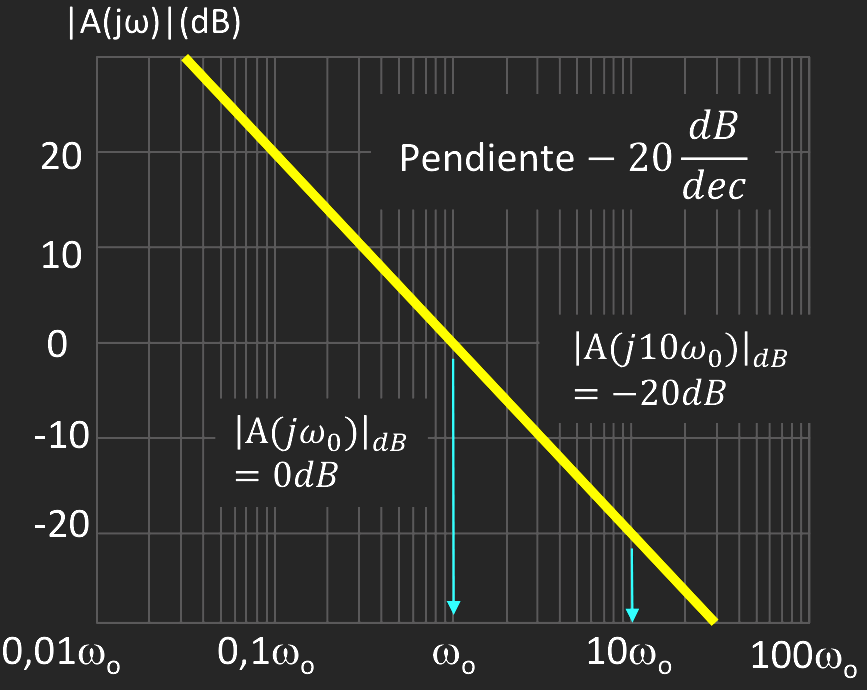
\includegraphics[width=\textwidth]{figbode231.jpg} 
\end{minipage}
\begin{minipage}{0.49\textwidth}
$$
\varphi [A (j \omega)] = -90^\circ
$$

\bigskip

    \centering
    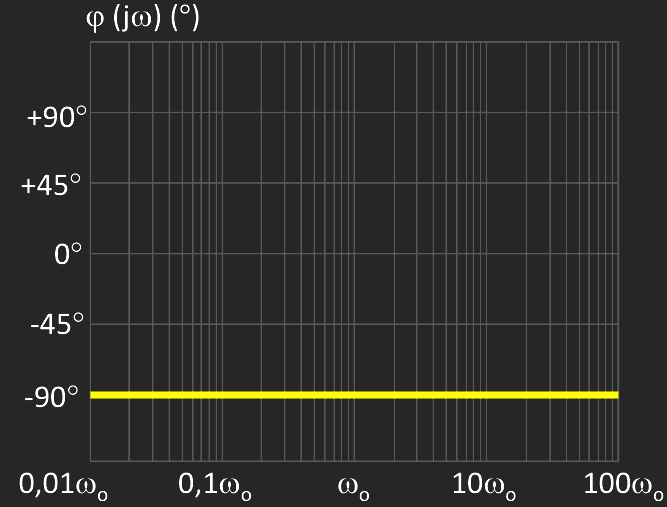
\includegraphics[width=\textwidth]{figbode232.jpg} 
\end{minipage}
\hrule
\subsection{Cero simple}
$$
A (j \omega) = 1 + j \frac{\omega}{\omega_0}
$$
\begin{minipage}{0.49\textwidth}
$$
|A (j \omega)| = \sqrt{1 + \left(\frac{\omega}{\omega_0}\right)^2}
$$
    \centering
    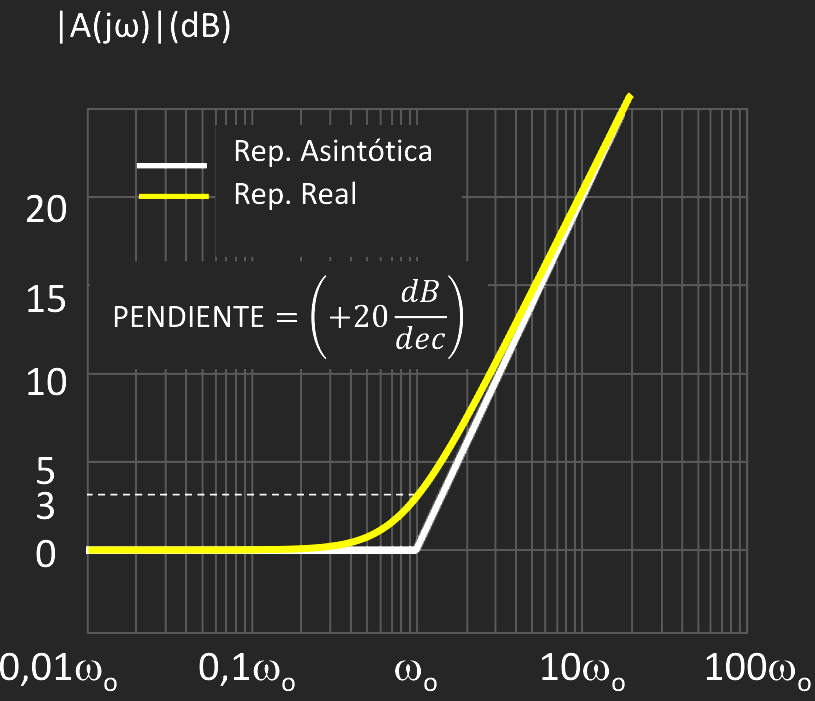
\includegraphics[width=\textwidth]{figbode241.jpg} 
\end{minipage}
\end{document}
